%%%%%%%%%%%%%%%%%%%%%%%%%%%%%%%%%%%%%%%%%
%%%%%%%%%% Content starts here %%%%%%%%%%
%%%%%%%%%%%%%%%%%%%%%%%%%%%%%%%%%%%%%%%%%

\begin{frame}{Contents}
	\begin{itemize}
	  \item Introduction
	  \item Methodology
	  \item Results
    \item Reports on plagiarism
	  \item Evaluation
    \item Conclusion
	\end{itemize}
\end{frame}

\begin{frame}{Introduction}
	\begin{itemize}
    \item 900 students in 2012
    \item 1029 students in 2013
	  \item \emph{Code} is a web-based system for automatic assessment of programming problems
	  \item Help insturctors in identified dificulties in assessing students' solutions
	  \item Also used in practical exams that involve programming assignments
	  \item Timed and informative feedback and automatic assessment is top priority
	\end{itemize}
\end{frame}

\begin{frame}{Methodology}
    \begin{itemize}
      \item We analyze the data generated from the usage of the system at FCSE
      \item The system is in use from September 2012 in more than 10 courses that involve some kind of programming
      assignments in programming languages such as C, C++ or Java
      \item More than 1200 problems, 45\% are exams
      \item Students mostly work using the the web-based editor in introductionary courses and IDEs in more advanced courses
      \item Unlimited submissions and as many problem attempt records
    \end{itemize}
\end{frame}

\begin{frame}{Problems success rate}
    \begin{figure}
    \centering
        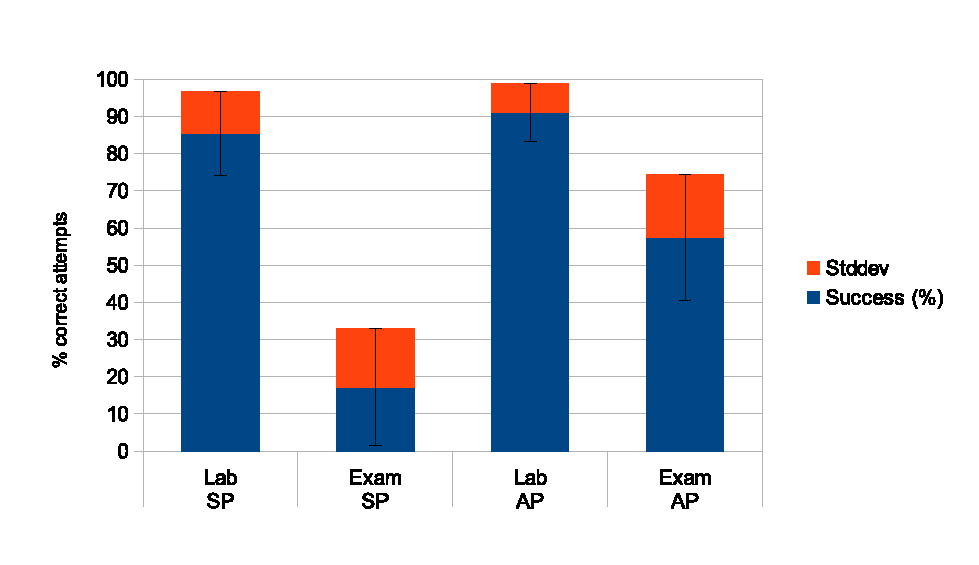
\includegraphics[width=.9\textwidth]{../code_usage/problems_success_rate}
        \caption{Problem success rate.}
        \label{fig:success_rate}
    \end{figure}
\end{frame}

\begin{frame}{Students success rate}
\begin{figure}
\centering
\begin{subfigure}{.5\textwidth}
  \centering
  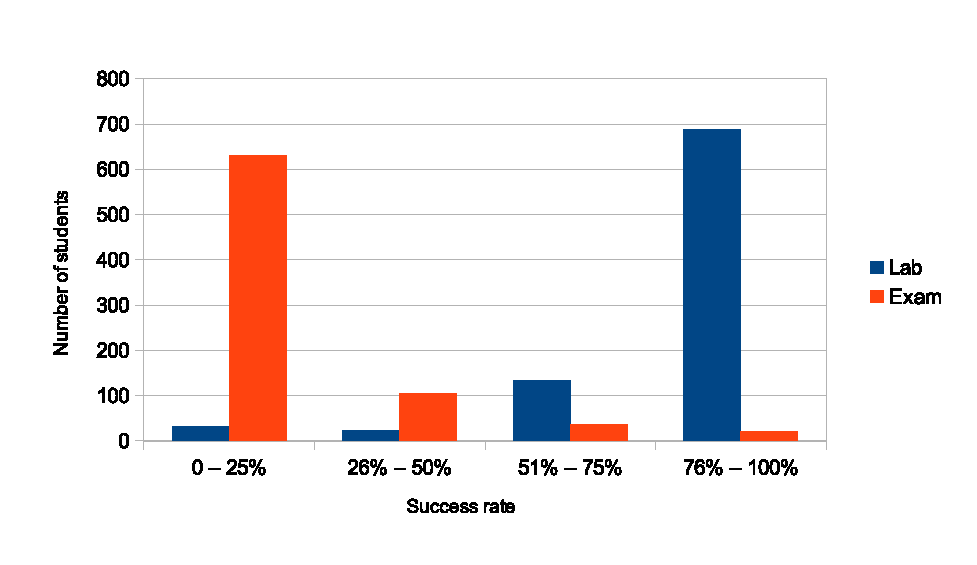
\includegraphics[width=\linewidth]{../code_usage/sp_success_rate}
  \caption{SP success rate}
  \label{fig:sp_success_rate}
\end{subfigure}%
\begin{subfigure}{.5\textwidth}
  \centering
  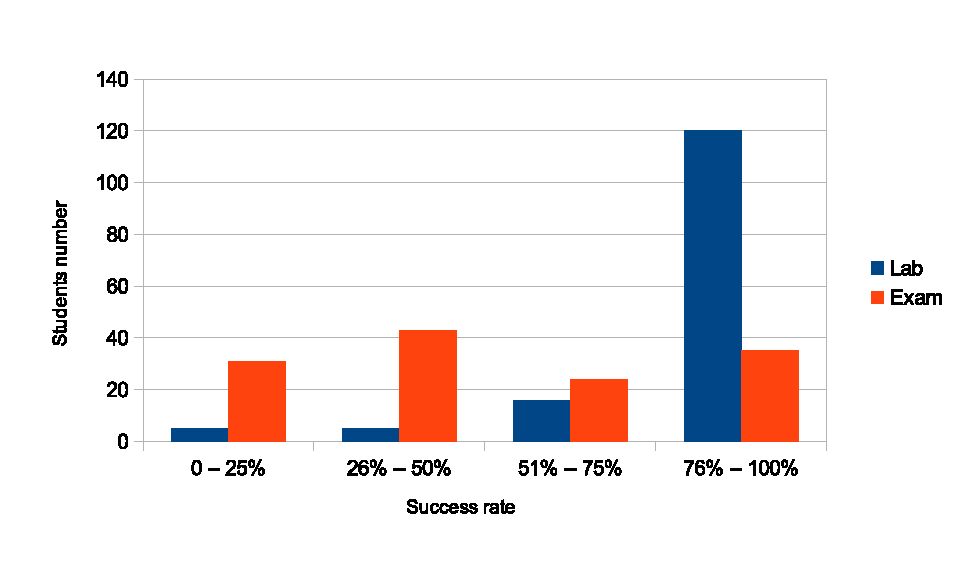
\includegraphics[width=\linewidth]{../code_usage/ap_success_rate}
  \caption{AP success rate}
  \label{fig:ap_success_rate}
\end{subfigure}
\caption{Success rate on students}
\label{fig:students_success_rate}
\end{figure}
\end{frame}


\begin{frame}[shrink=10]{Source code evolution}
\begin{table}
\caption{Source code evolution data}
\begin{center}
\begin{tabular}{ |p{1.5cm}|l|p{2cm}|p{1.5cm}|p{1.5cm}|p{1.5cm}| }
\hline
 \textbf{Problem} & & \textbf{Average delta time (seconds)} & \textbf{Average
 compile success} & \textbf{Average deltas} & \textbf{Average lines} \\
\hline
\multirow{2}{*}{Recursion} 
& Correct & 408.7 & 0.77 & 1.72 & 29.8 \\
\cline{2-6}
& Incorrect & 172.4 & 0.49 & 1.47 & 25.0 \\
\hline
\multirow{2}{*}{Matrix}
& Correct & 137.6 & 0.90 & 1.85 & 40.4 \\
\cline{2-6}
& Incorrect & 228.1 & 0.61 & 1.79 & 32.6 \\
\hline
\multirow{2}{*}{Files}
 & Correct & 75.8 & 0.64 & 1.19 & 52.5 \\
 \cline{2-6}
 & Incorrect & 484.5 & 0.58 & 1.26 & 49.4 \\
\hline
\end{tabular}
\label{table:code_evolution}
\end{center}
\end{table}
\end{frame}

\begin{frame}{Plagiarism}
  \begin{table}[htb]
  \caption{Results on plagiarism detection using MOSS}
  \begin{center}
  \begin{tabular}{ |l|p{2cm}|p{2cm}|p{2cm}|p{2cm}| }
  \hline
  Course & Settings & Average percentage match & Average lines matched & Potential
  plagiarism pairs
  \\
  \hline 
  \multirow{2}{*}{SP} & Lab & 52.04\% & 16.37 & 3869 \\
   & Exam & 22.74\% & 8.06 & 20 \\
  \hline
  \multirow{2}{*}{AP} & Lab & 10.08\% & 28.22 & 1 \\
   & Exam  & 10.26\% & 20.12 & 2 \\
  \hline
  \end{tabular}
  \label{table:plagiarism_results}
  \end{center}
  \end{table}
\end{frame}

\begin{frame}{Plagiarism example}
    \begin{figure}
    \centering
        \includegraphics[width=.9\textwidth]{../code_usage/plagiat_example}
        \caption{Plagiarism example.}
        \label{fig:plagiat_example}
    \end{figure}
\end{frame}

\begin{frame}{Evaluation}
    \begin{itemize}
      \item Group of 48 students in period of 10 days
      \item Three group of questions
      \begin{itemize}
      \item General questions
      \item System evaluation questions
      \item Learning programming questions
      \end{itemize}
    \end{itemize}
\end{frame}

\begin{frame}[shrink=20]{General usage questions}
\begin{table}
\caption{General usage questions}
\begin{center}
\begin{tabular}{ |p{5cm}|p{5cm}|l| }
\hline
\multirow{5}{*}{I used Code in?} & 1. Structured Programming (C) & 40\% \\
\cline{2-3}
 & 2. Object Oriented Programming (C++/Java) & 49\% \\
 \cline{2-3}
 & 3. Algorithms and Data Structures (C/Java) & 5\% \\
 \cline{2-3}
 & 4. Advanced Programming (Java) & 3\% \\
 \cline{2-3}
 & 5. Advanced Algorithms (Java) & 3\% \\
 \cline{2-3}
\hline
\multirow{2}{*}{I access Code from?} & 1. Faculty labs & 38\% \\
 & 2. From anywhere & 62\% \\
 \hline
\multirow{2}{5cm}{Do you want access from anywhere?} & Yes & 98\% \\
\cline{2-3}
 & No & 2\% \\
\hline
\multirow{4}{*}{How often do you use Code?} & 1. I don't use it & 1\% \\
\cline{2-3}
 & 2. Once a week & 42\% \\
 \cline{2-3}
 & 3. 2-3 times a week & 42\% \\
 \cline{2-3}
 & 4. More than 3 times a week & 15\% \\
 \cline{2-3}
\hline
\end{tabular}
\label{table:general_questions}
\end{center}
\end{table}
\end{frame}

\begin{frame}[shrink=20]{System evaluation questions}
\begin{table}
\caption{System evaluation questions (1-5 grades)}
\begin{center}
\begin{tabular}{ |p{5cm}|l|l|l|l|l| }
\hline
Simple to use? & 1 (0\%) & 2 (2\%) & 3 (10\%) & 4 (21\%) & 5 (67\%) \\
\hline
Quality of presentation in problem view? & 1 (0\%) & 2 (13\%) & 3 (6\%) & 4
(21\%) & 5 (60\%)
\\
\hline
Code editor functionality? & 1 (4\%) & 2 (13\%) & 3 (13\%) & 4 (40\%) & 5 (31\%)
\\
\hline
Performance and speed? & 1 (0\%) & 2 (6\%) & 3 (6\%) & 4 (31\%) & 5 (56\%) \\
\hline
Do you think Code helps you in correctly solving the problem? &
\multicolumn{3}{l|}{Yes (62\%)} & \multicolumn{2}{l|}{No (38\%)}
 \\
\hline
When using Code? & \multicolumn{2}{p{2.5cm}|}{First use IDE and then copy the
solution (83\%)} & \multicolumn{2}{p{2.5cm}|}{Use the web-based code editor
(13\%)} & Other (4\%) \\
\hline
\end{tabular}
\label{table:system_evaluation}
\end{center}
\end{table}
\end{frame}

\begin{frame}[shrink=20]{Learning programming}
\begin{table}[htb]
\caption{Learning programming}
\begin{center}
\begin{tabular}{ |p{4cm}|p{7cm}|l| }
\hline
\multirow{3}{4cm}{Where do you feel that you most learn (programming)?} &
1. Lectures & 4\%\\
\cline{2-3}
 & 2. TA Exams lectures & 17\% \\
 \cline{2-3}
 & 3. Lab exercises & 31\% \\
 \cline{2-3}
 & 4. Individual learning & 31\% \\
 \cline{2-3}
 & 5. Solving problems in Code & 5\% \\
 \cline{2-3}
 & 6. Other & 6\%\\
\hline
\multirow{3}{4cm}{What kind of materials helps you most in learning?} &
1. Books on subject & 13\%\\
\cline{2-3}
 & 2. Lectures slides & 15\% \\
\cline{2-3}
 & 3. Exercises questions and answers & 4\% \\
\cline{2-3} 
 & 4. Example problems with solutions & 46\% \\
 \cline{2-3}
 & 5. Interactive visualization of solutions & 13\% \\
 \cline{2-3}
 & 6. Other & 10\%\\
\hline
\multirow{3}{4cm}{While solving problem on code I mostly need help in?} &
1. Understand a problem and think of algorithm & 21\%\\
\cline{2-3}
 & 2. Implementing (coding) my solution & 27\% \\
 \cline{2-3}
 & 3. Locating and fixing errors in my solution & 46\% \\
 \cline{2-3}
 & 4. Other & 6\%\\
\hline
\multirow{3}{4cm}{What kind of help would be useful to be implemented?} &
1. Automatically showing relevant materials with similar problems and solutions
& 63\%\\
\cline{2-3}
 & 2. Direct communication with tutors over chat & 23\% \\
 \cline{2-3}
 & 3. Other & 7\%\\
\hline
\end{tabular}
\label{table:learning_programming}
\end{center}
\end{table}
\end{frame}


\begin{frame}{Questions}{}
    \begin{center}
    \Large{
    \href{http://code.finki.ukim.mk/}{\textbf{http://code.finki.ukim.mk}}}
    \vfill
    \huge{Thank You for the attention}
    \vfill    
    \Huge{Questions?}
    \end{center}
\end{frame}






